\chapter{Metodologia}\label{chp:met}

\section{Projeto}

\subsection{Necessidades}

\subsubsection{O cliente}
O cliente do presente projeto é a equipe Céu Azul Aeronaves, que representa anualmente a UFSC na competição SAE Brasil Aerodesign. A equipe desenvolve VANTs com missões variadas, mas que (em geral) giram em torno da maximização da eficiência estrutural da aeronave projetada[X]. O autor do presente texto trabalhou durante 5 anos na equipe e viu nesta necessidade a oportunidade de desenvolvimento do presente trabalho.

O objetivo da bancada é medir os coeficientes aerodinâmicos (de sustentação, arrasto e momento) em componentes dos VANTs desenvolvidos na equipe, além da medição de empuxo dinâmico em conjuntos moto-propulsores e a interação de seu escoamento com o restante da aeronave.

Para cumprir com o objetivo proposto, algumas necessidades foram levantadas:

\begin{enumerate}
    \item Tal bancada deve possuir rigidez suficiente para que suas medições sejam consistentes no tempo e a necessidade de manutenção seja baixa.
    \item Deve ser possível acoplar a bancada na caçamba de uma camionete ou ao rack de um carro comum, de modo a facilitar sua instalação.
    \item Levando em conta que a equipe sofre de alta rotatividade de membros e nem sempre é possível garantir que existirão pessoas capacitadas a trabalhar neste projeto é importante que a bancada em questão seja entregue na forma de um "produto final", isto é, funcione sem a necessidade de conhecimento de suas intrinsidade, com pouco mais que um manual de instruções e considerações para seu uso.
    \item Da mesma forma que o uso da bancada deve ser facilitado, também deve ser assim o uso dos dados fornecidos por ela. Idealmente se deseja que a mesma entregue os coeficientes finais, já processados, assim como suas incertezas de medição.
\end{enumerate}

\subsection{Considerações}

Assume-se para o presente projeto que o escoamento de ar que alcança a geometria analisada tem direção relativamente estável, é aproximadamente paralela ao deslocamento do veiculo e que a velocidade é praticamente constante para pequenos trechos a serem analisados.

Dado que a velocidade do veiculo é controlada por um piloto humano, oscilações da ordem de 10\% na velocidade são esperadas durante os patamares de velocidade e serão mensuradas através de tubos de Pitot.

\begin{figure}[!ht]
    \centering
    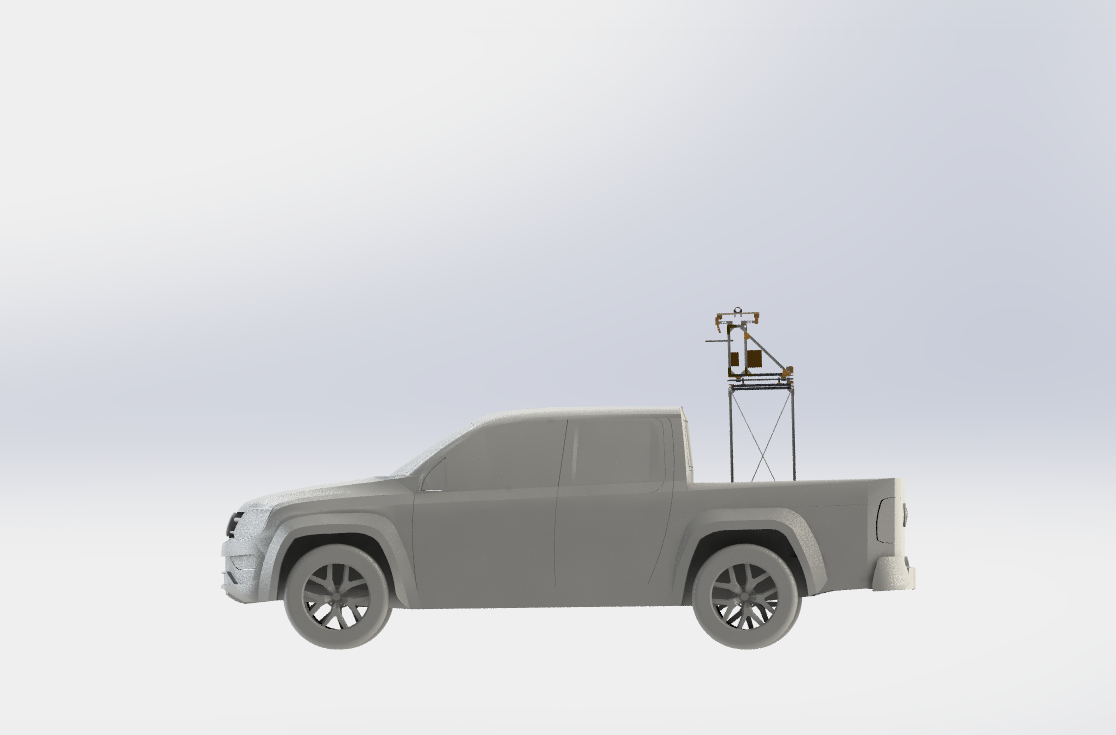
\includegraphics[width=.8\linewidth]{figuras/renders/bancada_no_carro_lateral.png}
    \caption{Angulo de escoamento induzido pela carenagem do carro sobre a região de medições\cite{autor}.}
    \label{fig:vehicle-angle}
\end{figure}

É possível também que a carroceria do veiculo induza um angulo diferente de zero ao escoamento que chega a bancada (ver \prettyref{fig:vehicle-angle}). Um Pitot de múltiplas tomadas sera instalado na bancada a fim de medir este angulo e ajustar os dados no pós-processamento. Eh importante ressaltar que tal sonda  possui limitação de operação de aproximadamente 15 graus em cada sentido[X], sendo assim, ângulos maiores que este não terão uma leitura adequada. Grandes desvios de angulo do escoamento ou velocidades muito instáveis provavelmente tornarão o processamento dos dados dos testes impeditivo e portanto cuidados devem ser tomados para que o teste se conduza de forma adequada.

\begin{figure}[!ht]
    \centering
    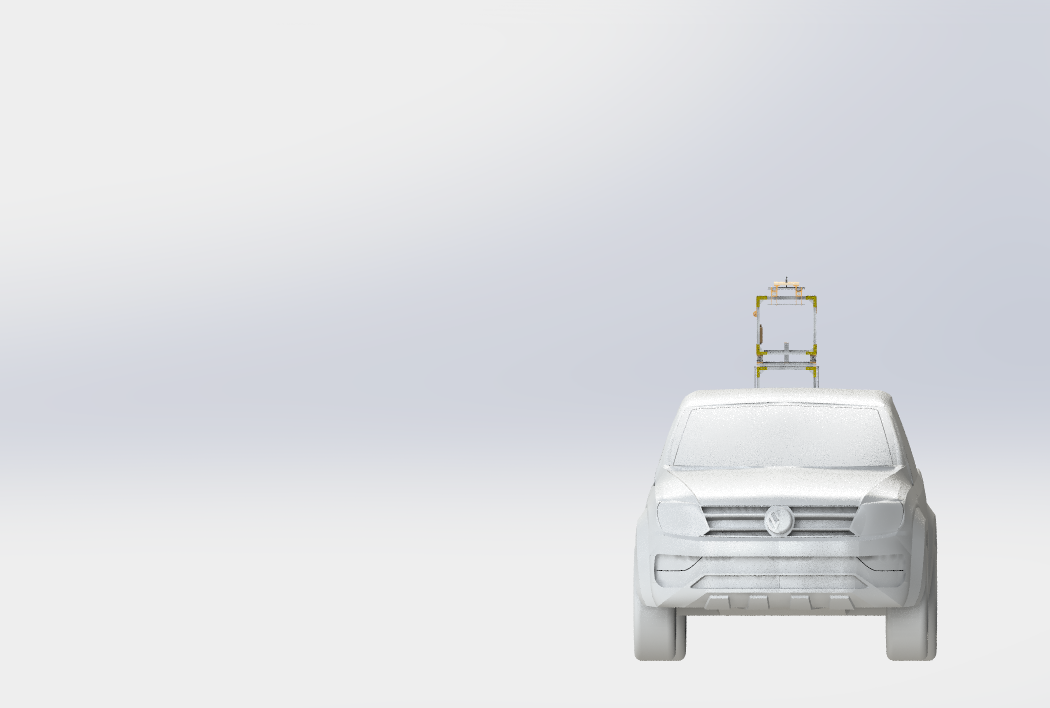
\includegraphics[width=.8\linewidth]{figuras/renders/bancada_no_carro_curva_frontal.png}
    \caption{Surgimento de força radial sob o componente quando em curva\cite{autor}.}
    \label{fig:forca_radial_frontal}
\end{figure}

\begin{figure}[!ht]
    \centering
    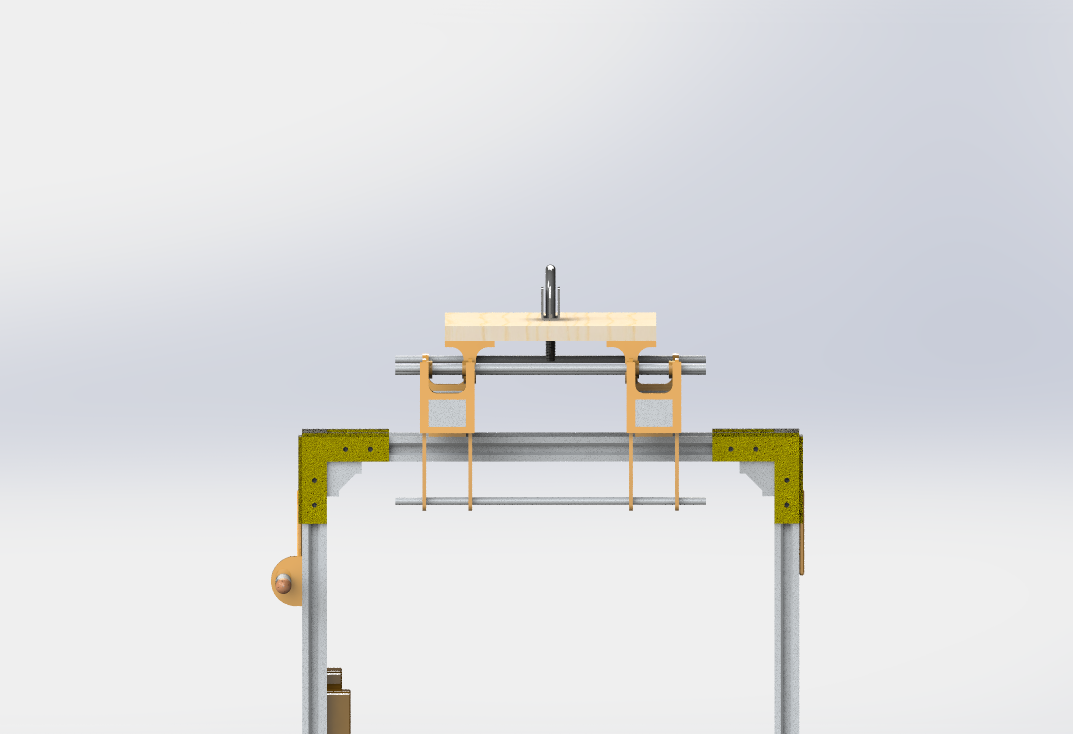
\includegraphics[width=.8\linewidth]{figuras/renders/carro_momento_roll_frontal.png}
    \caption{Momento de rolagem artificial medido quando em curva\cite{autor}.}
    \label{fig:momento_falso_roll}
\end{figure}

\begin{figure}[!ht]
    \centering
    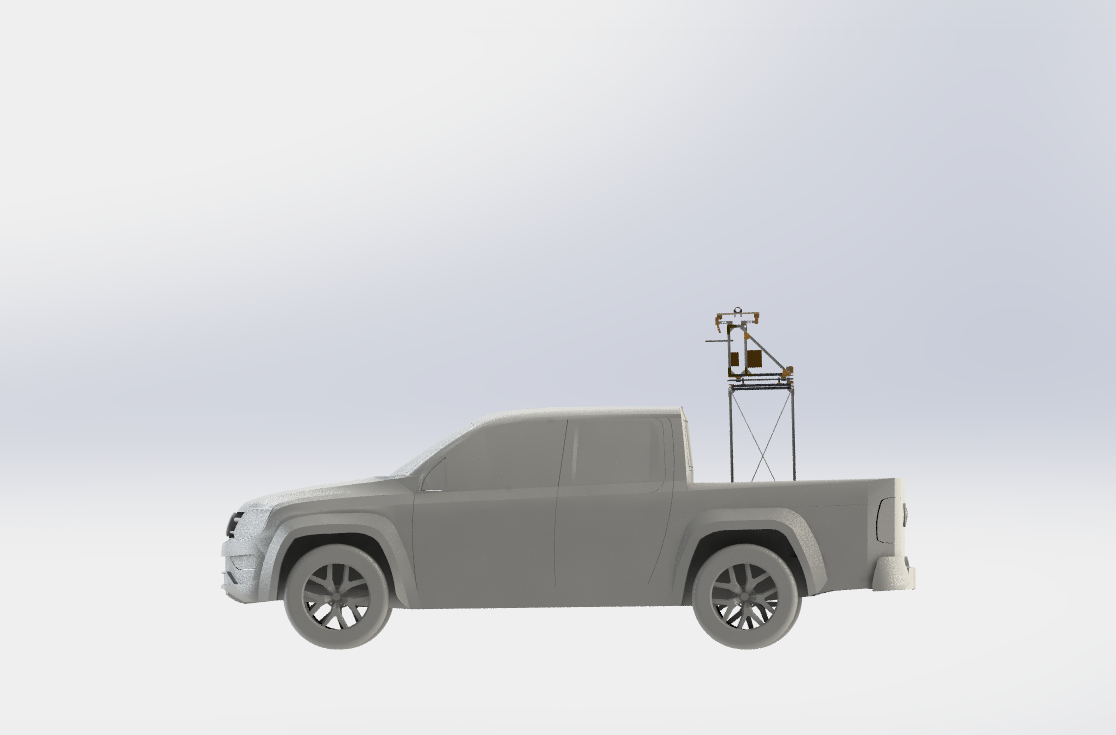
\includegraphics[width=.8\linewidth]{figuras/renders/bancada_no_carro_lateral.png}
    \caption{Oscilaçoes em pista causam erro na mediçao das forças e desalinhamento do escoamento\cite{autor}.}
    \label{fig:ocsilacoes_em_pista}
\end{figure}

Assume-se também que existem obstáculos na pista (tais como buracos e pequenas elevações), mas que de forma geral o teste sera conduzido em pistas relativamente retas e planas, de modo que não existam vibrações constantes ou acelerações radiais a serem modeladas no sistema. Pequenas oscilações serão medidas por acelerômetros e giroscópios e levadas em conta também no pós-processamento.

\subsection{Estimativas}

Para os projetos mecânico e eletrônico foram estimadas situações extremas de medição e para estas a bancada foi dimensionada:

\begin{itemize}
    \item Caracterização de aeronave completa com até 300N de sustentação, 50N de arrasto e XXXN de Momento
    \item Caracterização de conjunto motopropulsor com até 70N de empuxo estático
    \item Escoamentos com velocidade de até 25m/s
    \item Fatores de carga na bancada de até 4g
\end{itemize}

\subsection{Solução proposta}

A solução proposta consiste em uma bancada sensoriada, montada sobre uma estrutura metálica que a eleve até a altura desejada para o teste.

O veiculo a ser utilizado nos testes é do modelo Volkswagen Amarok 2017, tendo a caçamba uma altura de XXX m e o teto do carro elevando-se XXX m acima da altura da caçamba.

\begin{figure}[!ht]
    \centering
    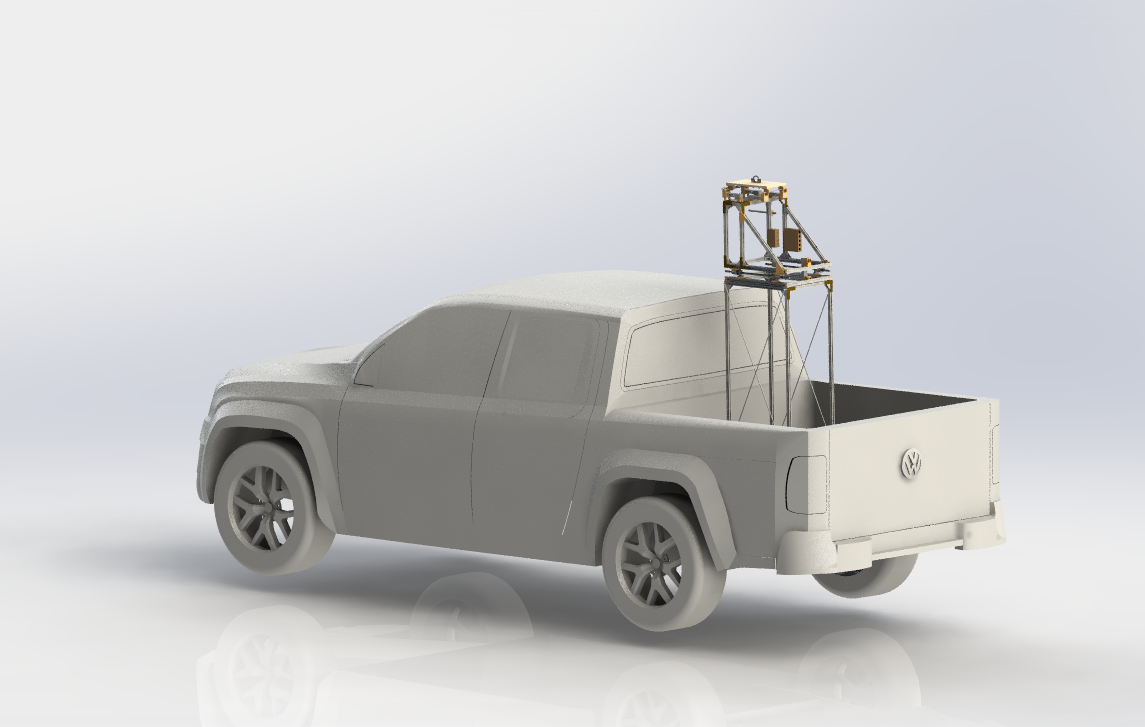
\includegraphics[width=.8\linewidth]{figuras/renders/bancada_no_carro_perspectiva.png}
    \caption{ESQUEMATICO DA BANCADA + TORRE\cite{autor}.}
    \label{fig:placeholder}
\end{figure}

\subsubsection{Sensoriamento das forças}

As forças na bancada são sensoriadas por quatro células de cargas verticais e uma célula de carga horizontal. A célula horizontal permite medição do arrasto/empuxo, o somatório das células verticais permitem a medição da sustentação, a diferença entre as células frontais e traseiras permite a medição do momento de picada (pitch) e a diferença entre as células da esquerda e da direita permite a medição do momento de rolagem (roll).

\begin{figure}[!ht]
    \centering
    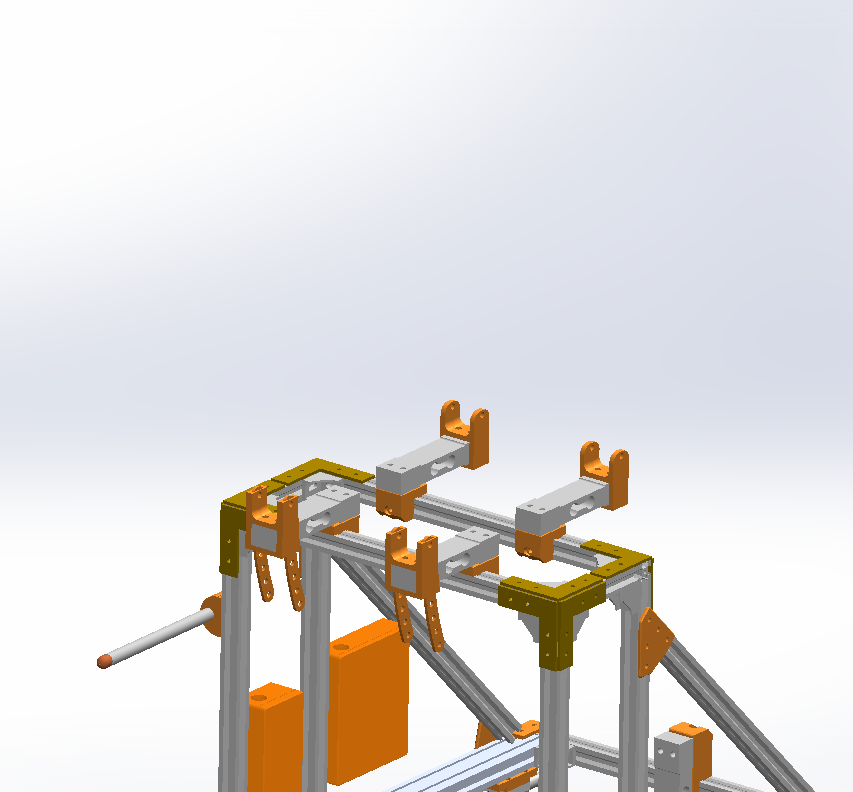
\includegraphics[width=.8\linewidth]{figuras/renders/esquematico_celulas_lift.png}
    \caption{Leitura de sustentação\cite{autor}.}
    \label{fig:leitura_sustentacao}
\end{figure}

\begin{figure}[!ht]
    \centering
    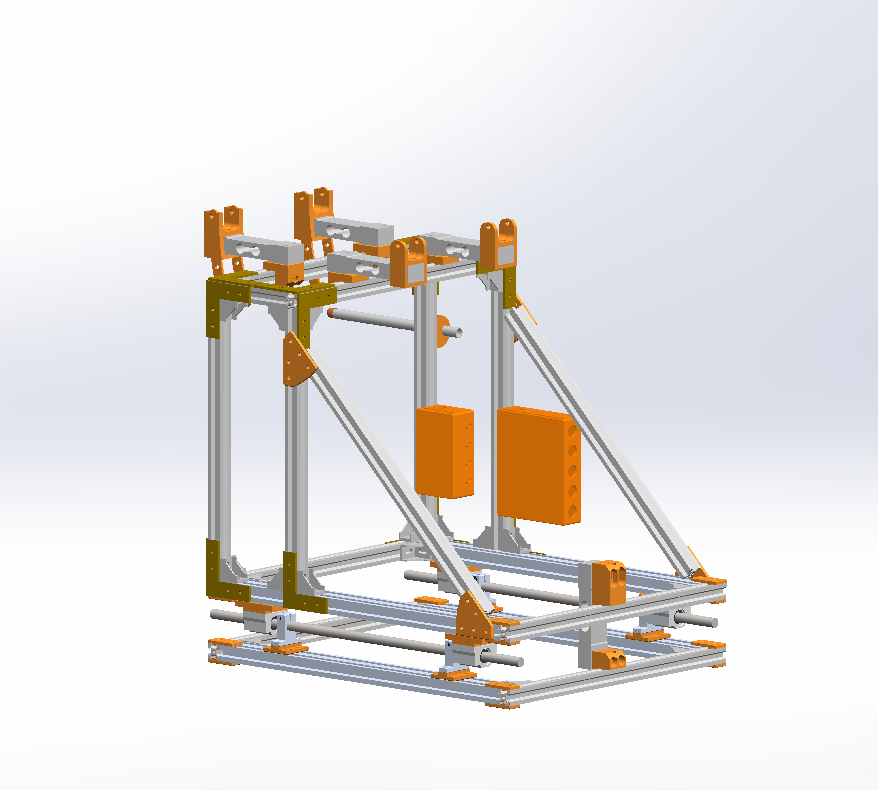
\includegraphics[width=.8\linewidth]{figuras/renders/esquematico_celulas_drag_2.png}
    \caption{Leitura de arrasto\cite{autor}.}
    \label{fig:leitura_arrasto}
\end{figure}

\begin{figure}[!ht]
    \centering
    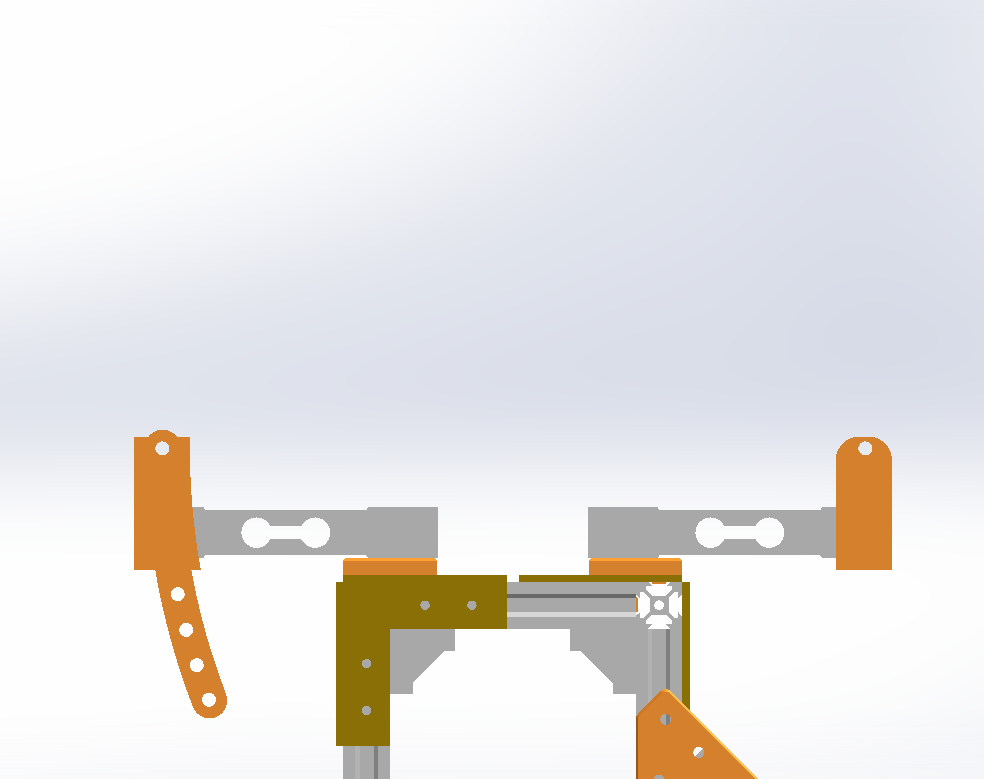
\includegraphics[width=.8\linewidth]{figuras/renders/esquematico_celulas_momento_pitch.png}
    \caption{Leitura de momento de picada\cite{autor}.}
    \label{fig:leitura_momento_pitch}
\end{figure}

\begin{figure}[!ht]
    \centering
    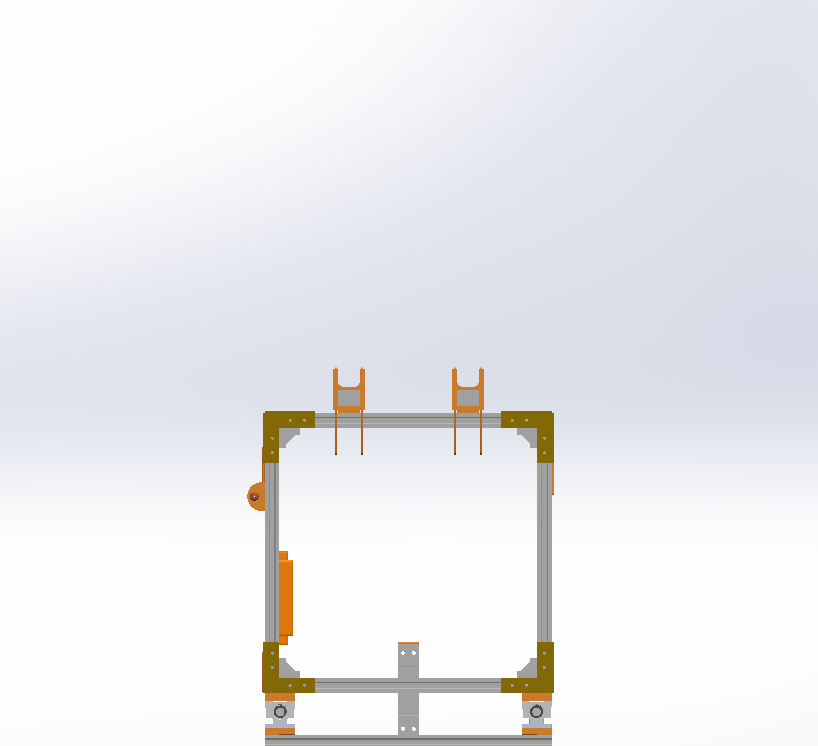
\includegraphics[width=.8\linewidth]{figuras/renders/esquematico_celulas_momento_roll.png}
    \caption{Leitura de momento de rolagem\cite{autor}.}
    \label{fig:leitura_momento_roll}
\end{figure}

\subsubsection{Sensoriamento de velocidade e angulo de ataque}

Ainda na bancada serão instalados um tubo de Pitot e um Pitot de múltiplas tomadas (sonda de angulo de ataque). Ambos serão instalados o mais próximo possível ao escoamento livre. Enquanto o Pitot sera acoplado a própria bancada, a sonda ficara alinhada com o eixo principal de picada do componente que estiver sendo analisado, de modo a medir o angulo de ataque real do mesmo. 

\begin{figure}[!ht]
    \centering
    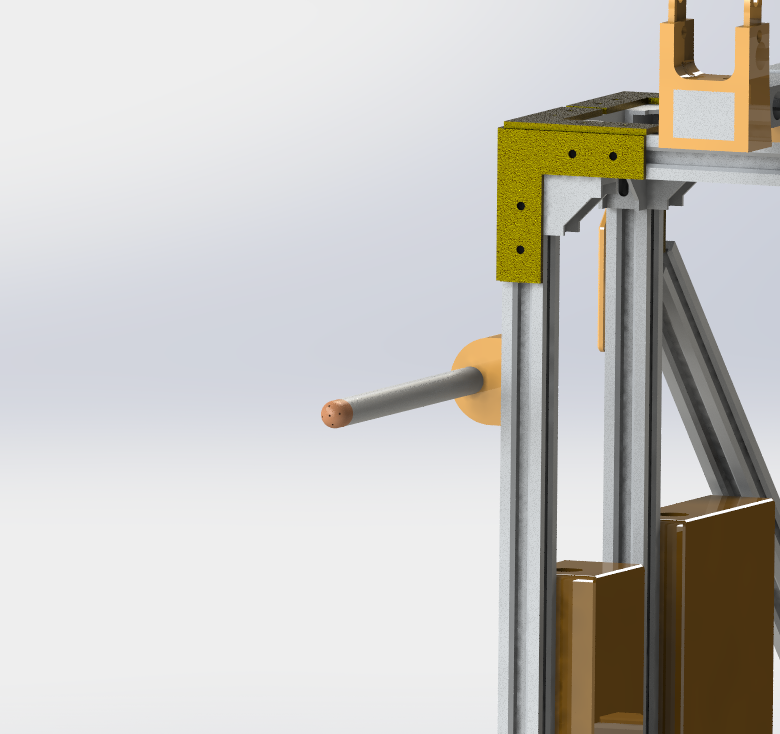
\includegraphics[width=.8\linewidth]{figuras/renders/detalhe_pitot_bancada.png}
    \caption{Posicionamento do tubo de Pitot na bancada para medição da velocidade de fluxo livre \cite{autor}.}
    \label{fig:placeholder}
\end{figure}

\begin{figure}[!ht]
    \centering
    
\includegraphics[width=.8\linewidth]{figuras/outras/placeholder.png}
    \caption{IMAGEM DA SONDA NA ASA \cite{autor}.}
    \label{fig:placeholder}
\end{figure}

O sistema deve comportar ainda a adição de novos sensores de forma a permitir a caracterização do escoamento em outros pontos de interesse, como esteira da hélice ou escoamento incidente no profundor.

\begin{figure}[!ht]
    \centering
    
\includegraphics[width=.8\linewidth]{figuras/outras/placeholder.png}
    \caption{IMAGEM DE PITOT NO PROFUNDOR \cite{autor}.}
    \label{fig:placeholder}
\end{figure}

\subsubsection{Sensoriamentos adicionais}

Para a medição do fator de carga vertical, assim como da temperatura e pressão do ar, uma Unidade de Medição Inercial (IMU) com acelerômetro, giroscópio, barômetro e termômetro será instalada na bancada.

\begin{figure}[!ht]
    \centering
    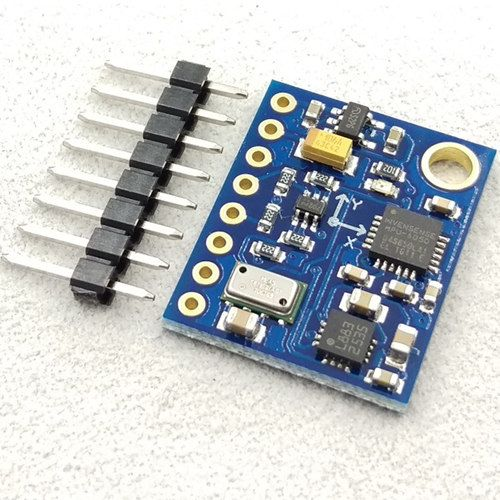
\includegraphics[width=.8\linewidth]{figuras/internet/IMU.jpg}
    \caption{Unidade de Medição Inercial (IMU) utilizada na bancada\cite{autor}.}
    \label{fig:placeholder}
\end{figure}

\subsubsection{Estação de controle e software de processamento}

Num primeiro momento foi levantada a possibilidade de se utilizar um computador portátil como estação de controle da bancada. Avaliou-se porém que isto poderia tornar o uso dificultado, já que em geral estes computadores possuem baterias que permitem poucas horas de uso continuo, limitando o tempo de execução de teste, além de serem relativamente grandes e pouco práticos de se utilizar dentro do carro.

De forma a facilitar o uso da bancada todo o controle do sistema foi projetado para ser realizado através de um aplicativo para celular. Nele é possível controlar a execução do teste, inserir informações para posterior avaliação, assim como acompanhar as medições dos sensores em tempo real, de modo a identificar possíveis problemas de forma rápida.

\begin{figure}[!ht]
    \centering
    
\includegraphics[width=.8\linewidth]{figuras/outras/placeholder.png}
    \caption{TELA DO APLICATIVO 1\cite{autor}.}
    \label{fig:tela_aplicativo_1}
\end{figure}

\begin{figure}[!ht]
    \centering
    
\includegraphics[width=.8\linewidth]{figuras/outras/placeholder.png}
    \caption{TELA DO APLICATIVO 2\cite{autor}.}
    \label{fig:tela_aplicativo_2}
\end{figure}

\begin{figure}[!ht]
    \centering
    
\includegraphics[width=.8\linewidth]{figuras/outras/placeholder.png}
    \caption{TELA DO APLICATIVO 3\cite{autor}.}
    \label{fig:tela_aplicativo_3}
\end{figure}

Será desenvolvido ainda um software de tratamento e analise de dados com interface gráfica e uso facilitado, este a ser utilizado em computador, devido a maior flexibilidade do mesmo para trabalhos longos.

\section{Projeto Mecânico}

Para o projeto mecânico foram levantadas as seguintes necessidades:

\begin{itemize}
    \item Facilidade construtiva, de forma a tornar rápida a construção e manutenção da bancada
    \item Baixo peso, de modo a não se criar uma barreira quanto ao uso da mesma
    \item Baixo arrasto aerodinâmico, a fim de diminuir a influência da estrutura nas medições
    \item Rigidez, para que as forças e momentos medidos sejam correspondentes aos modelados
    \item Baixo custo
\end{itemize}

Uma solução que responde de forma positiva a maioria dessas necessidades é a de uma estrutura composta de perfis extrudados de alumínio. Este tipo de estrutura é comumente encontrada em laboratórios ou fabricas, sendo utilizada para a construção de bancadas experimentais e estações de trabalho.

\begin{figure}[!ht]
    \centering
    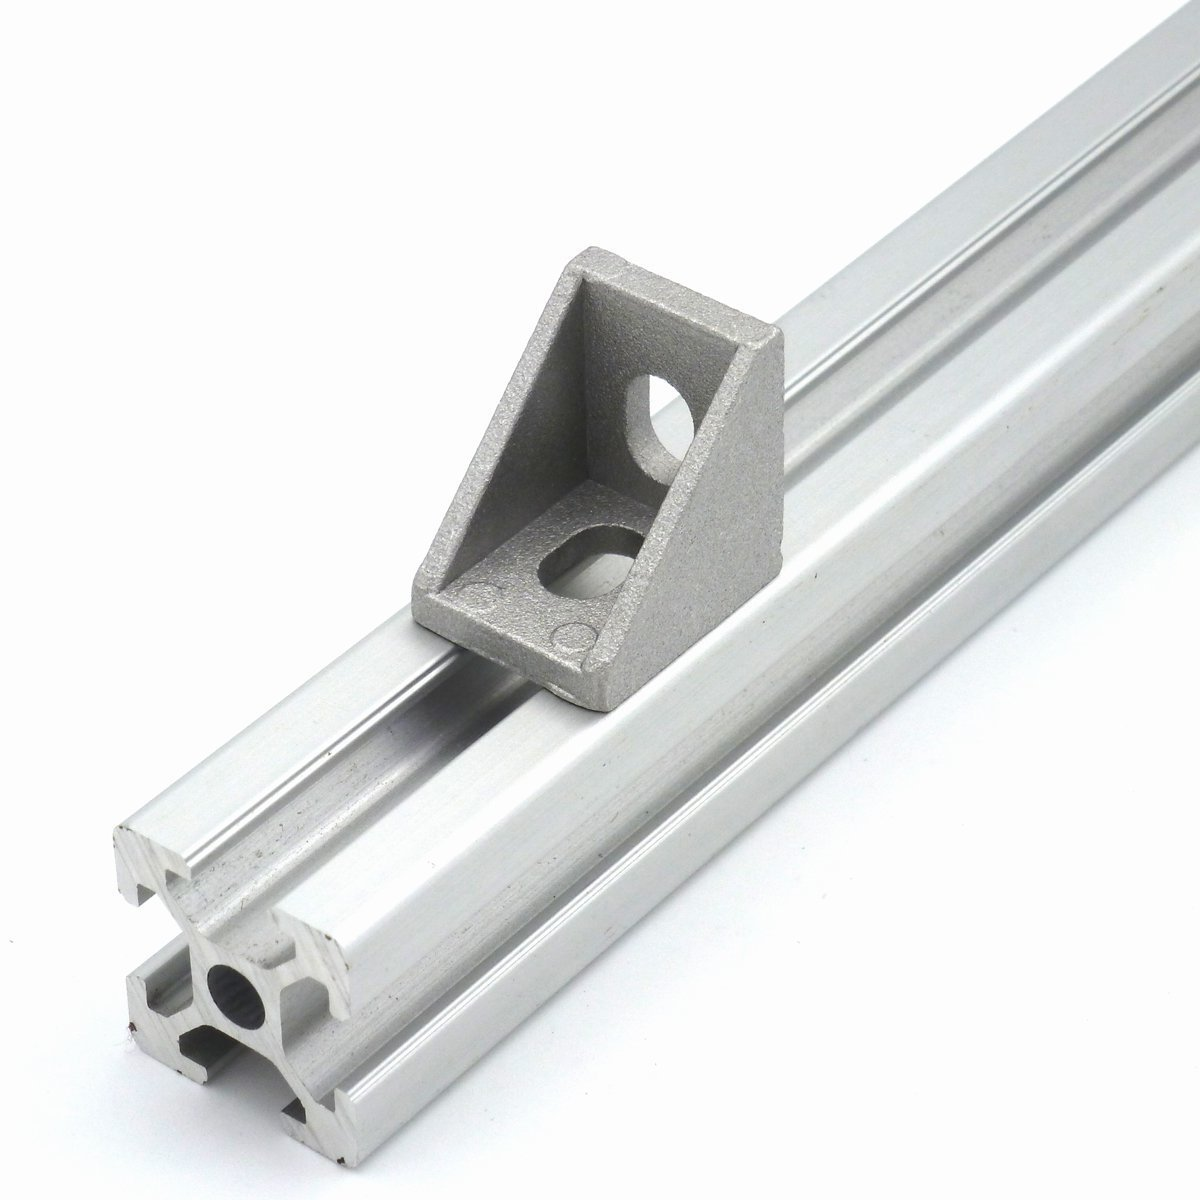
\includegraphics[width=.8\linewidth]{figuras/internet/perfil_aluminio.jpg}
    \caption{Perfil extrudado em alumínio utilizado na construção da bancada\cite{autor}.}
    \label{fig:perfil_aluminio}
\end{figure}

A desvantagem desta estrutura fica no provável alto arrasto aerodinâmico. Este porém é um problema contornável posteriormente carenando-se a estrutura. Ainda assim, com ou sem carenagem, este arrasto deve ser levado em conta nos testes e a maneira levantada de se mensurar esta grandeza é realizar os testes sem um componente a ser medido, medindo-se assim o arrasto aerodinâmico da própria bancada para que se possa descontar este valor das medições posteriores.

De modo a se medir o arrasto, duas soluções foram consideradas: 

\begin{enumerate}
    \item Uma célula de carga horizontal, tendo a bancada liberdade de movimento no eixo X
    \item Três células de carga restringindo completamente os graus de liberdade da bancada
\end{enumerate}

\begin{figure}[!ht]
    \centering
    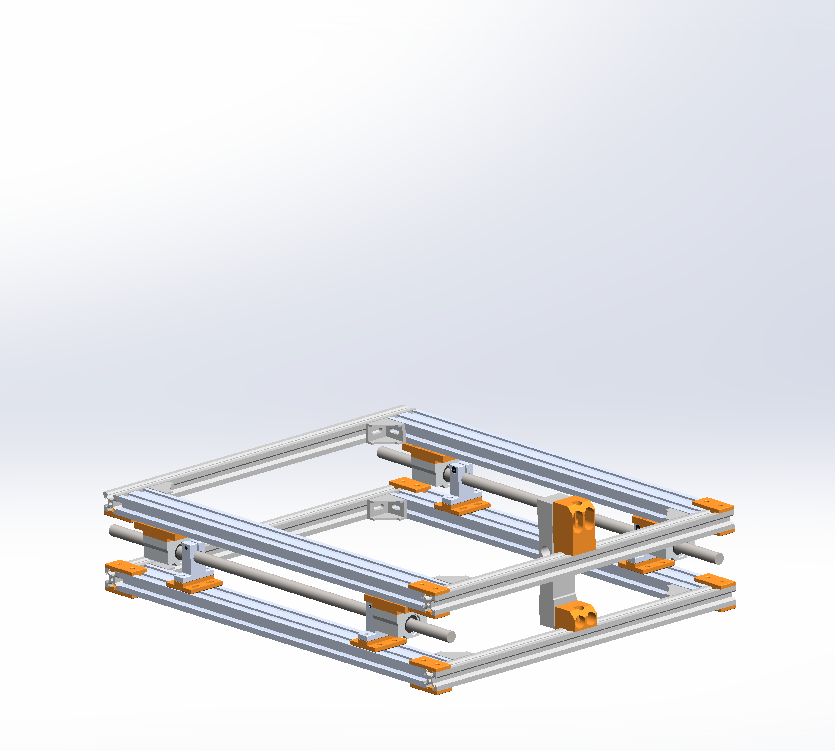
\includegraphics[width=.8\linewidth]{figuras/renders/bandeja_inferior.png}
    \caption{Solução para a medição de arrasto utilizando apenas uma célula de carga\cite{autor}.}
    \label{fig:bandeja_inferior_1}
\end{figure}

\begin{figure}[!ht]
    \centering
    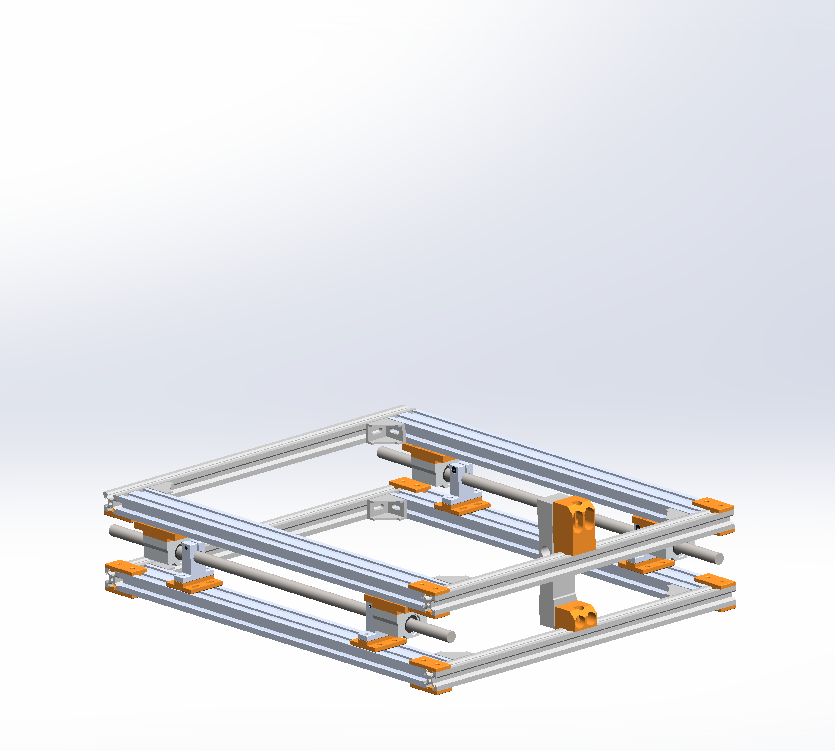
\includegraphics[width=.8\linewidth]{figuras/renders/bandeja_inferior.png}
    \caption{Solução para a medição de arrasto utilizando três células de carga TROCAR FOTO PRA 3 CELULASSS\cite{autor}.}
    \label{fig:bandeja_inferior_2}
\end{figure}

Devido ao fato de que a segunda solução exigiria ao menos três células de carga e as colocaria como componentes estruturais (já que não existiria outra ligação estrutural entre a parte inferior e superior da bancada) a primeira opção foi escolhida.

Para dar liberdade de movimentação no eixo X um conjunto de guias lineares e fixações rolamentadas foi escolhido, devido a seu baixo atrito e baixo custo. A desvantagem desta solução com apenas uma célula de carga se da justamente devido a existência desta força de atrito das guias no eixo X, que a principio não é medida. Esta força pode porem ser avaliada num primeiro momento, em laboratório, e compensada posteriormente.
    
\section{Projeto Eletrônico}

Para o sistema eletrônico da bancada tomou-se como ponto de partida a telemetria T2016, desenvolvida pela equipe Céu Azul inicialmente para utilização nos projetos da classe Advanced.

TROCAR TEXTO ABAIXO POR TABELA

Tal sistema consiste de um computador central, modelo Raspberry Pi 3 B+, rodando um sistema operacional Linux, com sensores conectados como periféricos. Entre os sensores já disponíveis na equipe estavam:

\begin{itemize}
    \item Tubos de Pitot com transdutores MPVX7002DP
    \item Modulo GNSS modelo uBlox NEO-6M
    \item IMU modelo GY-86, com acelerômetro de 3 eixos, giroscópio de 3 eixos, magnetômetro de 3 eixos, barômetro e termômetro
\end{itemize}

Além destes sensores o sistema possui um par de rádios seriais de 433MHz, que pode ser utilizado para transmissão dos dados em tempo real para o celular, comunicando a bancada com o aplicativo controlado pelo operador.

Para a medição das forças na bancada foi necessária a aquisição de células de carga e transdutores de célula de carga. Devido ao baixo custo optou-se por células sem marca. Esta decisão implica contudo num custo extra de tempo para a caracterização das células.

Para a transdução dos dados da célula (de resistência para tensão e posteriormente para força) foram adquiridos módulos HX711. Estes módulos são bastante comuns no mercado e implementam num mesmo CI a alimentação e leitura da ponte de Wheatstone, além da conversão dos dados analógicos em dados digitais. A maior vantagem deste CI é provavelmente a alimentação integrada da ponte de Wheatstone, por ser previamente estabilizada e filtrada, resultando em uma alta relação sinal-ruido. Em geral essa alimentação acontece em circuitos discretos separados do CI de leitura, e acabam resultando numa pior relação sinal-ruido.

\section{Projeto de Software Embarcado}

O software que roda de forma embarcada na plataforma central consiste em uma serie de módulos escritos em Python com funções desmembradas. Entre as funções necessárias no software destacam-se:

\begin{itemize}
    \item Aquisição de dados dos sensores
    \item Parseamento dos dados para padrão comum
    \item Transmissão serial de dados via radio
    \item Recebimento e interpretação de comandos externos
    \item Gravação dos dados no sistema
    \item Coordenação e sincronia dos processos anteriores
\end{itemize}

A figura X mostra a arquitetura do software divida em seus diversos módulos.

\begin{figure}[!ht]
    \centering
    
\includegraphics[width=.8\linewidth]{figuras/outras/placeholder.png}
    \caption{ESQUEMATICO DO SOFTWARE EMBARCADO\cite{autor}.}
    \label{fig:esquematico_software_embarcado}
\end{figure}

Este software já existia em versão primaria na plataforma T2016 e foi refatorado para uso na nova plataforma, permitindo que suas funções fossem estendidas. A totalidade das mudanças compreendidas por este trabalho pode ser vista no repositório Git do projeto [X]. 
\section{Projeto do Software de Analise}

O software de analise tem por função receber os dados "crus" gerados pela bancada e entregar dados uteis processados, com suas devidas incertezas estimadas.

Entre as características desejadas neste software estão:

\begin{itemize}
    \item Apresentar uma interface amigável para uso facilitado
    \item Receber os dados "crus"
    \item Filtrar cada dado conforme especificações previas ou personalizadas pelo usuário
    \item Apresentar os dados crus e processados na forma de gráficos
    \item Permitir interação do usuário com os dados
    \item Exportar os dados em formato útil, seja na forma textual, em planilhas ou mesmo diretamente como gráficos
\end{itemize}

A figura X mostra a arquitetura deste software.

\begin{figure}[!ht]
    \centering
    
\includegraphics[width=.8\linewidth]{figuras/outras/placeholder.png}
    \caption{ESQUEMATICO DO SOFTWARE DE ANALISE\cite{autor}.}
    \label{fig:esquematico_software_analise}
\end{figure}
